\chapter{Experimentación y Análisis de Resultados}
\label{chap:experimentacion}

Descritas en el capítulo anterior las arquitecturas de Word2Vec y QWord2Vec, este capítulo recoge el proceso de experimentación llevado a cabo para comparar ambos modelos de forma empírica. El objetivo central es evaluar si los \textit{embeddings} generados por QWord2Vec son capaces de preservar relaciones semánticas entre palabras con una calidad comparable a la de Word2Vec, entrenando cada modelo con las mejores técnicas disponibles dentro de su propio paradigma.

A lo largo del capítulo se argumentan las decisiones de diseño adoptadas (selección del corpus, elección de hiperparámetros, estrategias de entrenamiento y métricas de evaluación), diferenciando en cada caso correspondiente la aproximación seguida aquí de la propuesta en el trabajo de referencia \cite{ohno_qword2vec_2025} y analizando el efecto de las modificaciones introducidas. El objetivo no es reproducir el experimento original, sino explorar qué puede ofrecer cada modelo cuando opera bajo sus mejores condiciones pero partiendo de una base de referencia.

La experimentación se estructura en dos fases. La primera emplea el mismo corpus del artículo de referencia, lo que permite situar los resultados en un contexto comparable (aunque el objetivo final difiera ligeramente). La segunda introduce un corpus un poco más ampliado y equilibrado para analizar en qué medida la calidad de los datos de entrenamiento condiciona el rendimiento de cada modelo.

\section{Metodología experimental}

A continuación se describen los pasos previos necesarios para llevar a cabo la experimentación. En primer lugar, se presenta el corpus empleado para el entrenamiento de ambos modelos, junto con el proceso de preprocesamiento aplicado en cada caso. Al finalizar la explicación, se detallarán las herramientas y el entorno de ejecución utilizados, aspecto especialmente relevante en el caso de QWord2Vec, dado que la simulación clásica de circuitos cuánticos impone restricciones significativas sobre el tamaño del experimento realizable.

\subsection{Dataset y preprocesamiento}

Como se comentó anteriormente, la simulación clásica de circuitos cuánticos impone restricciones severas sobre el tamaño del experimento. A diferencia de Word2Vec clásico, que habitualmente se entrena con corpus de millones de frases y vocabularios de cientos de miles de palabras. El coste computacional de simular un circuito cuántico crece exponencialmente con el número de qubits, lo que hace inviable trabajar con corpus de gran escala en un equipo personal que es con el que se ha trabajado.

Por este motivo, la primera prueba de experimentación ha sido adoptando el mismo corpus empleado en el trabajo de referencia \cite{ohno_qword2vec_2025}, el cual fue tomado originalmente de una fuente web la cual ofrecía corpus pequeños para realizar evaluaciones de modelos de este estilo. El corpus consta de 13 frases en inglés con un vocabulario de 13 palabras únicas. Las frases utilizadas son las siguientes:

\begin{quote}
  \ttfamily
  i like dog \quad i like cat \quad i like animal \quad dog cat animal \\
  apple cat dog like \quad dog fish milk like \quad dog cat eyes like \\
  i like apple \quad apple i hate \quad apple i movie \\
  book music like \quad cat dog hate \quad cat dog like
\end{quote}

Las frases tienen una longitud de entre 3 y 4 palabras, lo que condiciona el tamaño de la ventana de contexto haciendo que sea pequeña. Desde el punto de vista de la distribución léxica, el corpus presenta un desequilibrio: las cuatro palabras más frecuentes (\textit{like}, \textit{dog}, \textit{cat} e \textit{i}) concentran el 67\% de los tokens totales, mientras que seis palabras del vocabulario aparecen una única vez. Este desequilibrio tiende a introducir distorsiones en las relaciones semánticas aprendidas por el modelo, y es una limitación que se asume de forma consciente.

No obstante, el uso de este corpus está justificado por tres razones. En primer lugar, permite reproducir directamente las condiciones experimentales del paper de referencia, facilitando la comparación de resultados durante el desarrollo e implementación de variaciones que se han realizado. En segundo lugar, el objetivo del estudio no es obtener un modelo de procesamiento del lenguaje natural de calidad, sino evaluar si QWord2Vec es capaz de preservar las relaciones semánticas que aprende Word2Vec. Para este fin, un corpus pequeño y controlado es suficiente. Por último, el tamaño reducido del vocabulario permite inspeccionar e interpretar los \textit{embeddings} obtenidos de forma directa, verificando manualmente que las relaciones semánticas resultantes son coherentes con el contenido del corpus.

En lo relativo al preprocesamiento del texto, no ha sido necesario aplicar ninguna técnica adicional sobre el conjunto de datos original. Esto se debe a que el corpus de experimentación es un conjunto ya preprocesado. Todas sus oraciones están escritas en minúsculas, no tienen signos de puntuación o caracteres especiales, y sus términos están delimitados por espacios simples. Por consiguiente, las etapas clásicas del procesamiento del lenguaje natural resultan redundantes, permitiendo que la separación básica por espacios genere directamente los \textit{tokens} esperados para la etapa de entrenamiento.

\subsection{Entorno de ejecución y herramientas}

Todos los experimentos se han llevado a cabo sobre un ordenador personal con sistema operativo Ubuntu, cuya compatibilidad con las librerías empleadas y su integración con el hardware disponible lo hacen especialmente adecuado para este tipo de desarrollo. Las características del hardware relevantes para el rendimiento son las siguientes:

\begin{itemize}
  \item \textbf{Procesador}: Intel Core i7-13700F (30\,MB de caché, frecuencia máxima superior a 5,2\,GHz).
  \item \textbf{Memoria RAM}: 32\,GB DDR4 a 3600\,MHz.
  \item \textbf{Tarjeta gráfica}: MSI GeForce RTX 4070 con 12\,GB de memoria GDDR6X.
\end{itemize}

En cuanto al software, las herramientas y librerías principales utilizadas en el desarrollo son:

\begin{itemize}
  \item \textbf{Python} 3.10.12: lenguaje de programación base del proyecto en el que se han desarrollado las implementaciones de ambos algoritmos.
  \item \textbf{Gensim} 4.4.0: empleada para el modelo clásico. Esta librería incluye tanto la arquitectura de Word2Vec como la función de optimización \textit{Negative Sampling}, desarrollada siguiendo las especificaciones originales de Google.
  \item \textbf{Qiskit} 1.4.5: utilizada para la versión cuántica. Proporciona las herramientas necesarias para la construcción del circuito parametrizado, la aplicación del optimizador y utilidades para la medición y transpilación del circuito. Frente a \textit{Qibo 0.2.11}, la librería empleada en el artículo de referencia \cite{ohno_qword2vec_2025}, se ha optado por \textit{Qiskit} por dos razones principales. En primer lugar, incorpora una implementación nativa del algoritmo \textit{QN-SPSA}, el optimizador elegido en este trabajo frente al \textit{SPSA} básico del artículo de referencia. En segundo lugar, ofrece una integración más madura con \textit{AerSimulator}, el \textit{backend} de simulación descrito a continuación.
  \item \textbf{Qiskit Aer} 0.17.2: \textit{backend} de simulación cuántica sobre hardware clásico.
\end{itemize}

Respecto a la elección del simulador cuántico, \textit{Qiskit} ofrece tres opciones: \textit{AerSimulator}, \textit{StatevectorSimulator} y \textit{QasmSimulator}. Los dos últimos se encuentran en proceso de deprecación, dado que \textit{AerSimulator} los unifica y supera en capacidades siendo el que más soporte y desarrollo recibe en la actualidad. Por este motivo, se ha optado por \textit{AerSimulator} como backend de simulación para la ejecución de QWord2Vec.

\subsection{Configuración de hiperparámetros}

Tanto el modelo clásico como el cuántico presentan una serie de hiperparámetros que deben ajustarse para obtener el mejor rendimiento posible, como ocurre en cualquier problema de \gls{ml}. Para su configuración se ha empleado la técnica de búsqueda exhaustiva \textit{Grid Search} \cite{dremio_grid_2026}, implementada manualmente en ambos casos al no disponer de una implementación genérica compatible con los modelos utilizados.

La estrategia seguida ha consistido en identificar, a partir de la literatura y de experiencias previas en problemas similares que han comentado distintas personas en foros, un conjunto de valores de referencia para cada hiperparámetro. A partir de estos valores, se han definido rangos de búsqueda que incluyen el valor de referencia junto con variaciones por encima y por debajo, con el objetivo de ajustar cada parámetro al corpus y al problema concreto. Dado que ambos modelos emplean funciones de pérdida y algoritmos de optimización distintos, cada uno dispone de su propio conjunto de hiperparámetros a explorar.

\subsection{Hiperparámetros de Word2Vec}

El artículo de referencia \cite{ohno_qword2vec_2025} implementó Word2Vec empleando la función de pérdida de entropía cruzada con softmax estándar como función de salida. En este trabajo, en cambio, se ha optado por \textit{Negative Sampling}, en línea con el objetivo descrito en la introducción de entrenar cada modelo con las mejores técnicas disponibles en su propio paradigma. Como se describió en el capítulo anterior, \textit{Negative Sampling} fue introducido y validado empíricamente por los propios autores de Google \cite{mikolov_skipgram_phrases_2013} como una alternativa superior al softmax en la mayoría de los escenarios de entrenamiento, convirtiéndose en la técnica de referencia en las implementaciones modernas de Word2Vec.

Los hiperparámetros de Word2Vec pueden agruparse en tres categorías ya que están los propios de la arquitectura Skip-Gram, los relacionados con \textit{Negative Sampling} y el correspondiente al optimizador.

En cuanto a los hiperparámetros de \textbf{Skip-Gram}, los dos parámetros ajustados son \textit{vector\_size} y \textit{window}. El primero determina la dimensionalidad de los vectores de \textit{embedding}, es decir, el número de características con el que se representa cada palabra. Su elección depende del tamaño del vocabulario, la riqueza semántica del corpus y los recursos computacionales disponibles. Dado que el vocabulario es de únicamente 13 palabras, no se requiere una representación de alta dimensionalidad para capturar las relaciones semánticas presentes. Por ello, se exploraron con solo dos valores que son el $\{2, 4\}$. El valor seleccionado por el \textit{Grid Search} fue $\text{vector\_size} = 2$, lo cual resulta coherente con el reducido tamaño del vocabulario y presenta la ventaja adicional de permitir visualizar directamente los \textit{embeddings} en el plano y realizar una validación manual sin necesidad de aplicar técnicas de reducción de dimensionalidad como PCA.

El segundo parámetro, \textit{window}, define la distancia máxima entre la palabra central y las palabras de contexto consideradas durante el entrenamiento, tal y como se ilustra en la Figura \ref{fig:window_ilustracion}. Los valores explorados fueron $\{1, 2\}$, teniendo en cuenta que las frases del corpus tienen entre 3 y 4 palabras. El valor seleccionado fue $\text{window} = 2$, la palabra central puede relacionarse con todas las demás en una frase de 4 palabras, mientras que si se hubiera elegido el tamaño 1, solo se consideraría la palabra adyacente.

\begin{figure}[h]
  \centering
  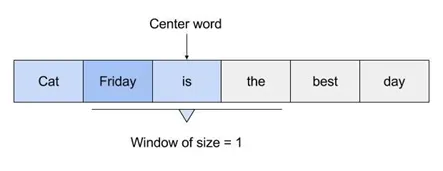
\includegraphics[width=0.7\linewidth]{imagenes/windowIlustration.png}
  \caption{Ilustración del parámetro \textit{window} en Skip-Gram: distancia máxima desde la palabra central hasta las palabras de contexto consideradas. Fuente: \cite{ali_word2vec_2019}.}
  \label{fig:window_ilustracion}
\end{figure}

Respecto a los hiperparámetros de \textbf{Negative Sampling}, los parámetros explorados son \textit{negative} y \textit{ns\_exponent}. El primero indica el número de muestras negativas que se generan por cada par positivo durante el entrenamiento. El artículo original publicado por Google \cite{mikolov_skipgram_phrases_2013} recomendó valores entre 5 y 20 (siendo 20 para corpus de gran escala). Dado que el corpus empleado cuenta únicamente con 13 palabras únicas, se optó por explorar valores ligeramente inferiores al valor mínimo que recomendaba el artículo de Google. Estos valores fueron el $\{2, 3\}$ siendo seleccionado $\text{negative} = 2$.

El parámetro \textit{ns\_exponent} controla la distribución de probabilidad con la que se seleccionan las palabras negativas. Un valor de 1 desfavorece a las palabras poco frecuentes respecto a una distribución puramente proporcional a las frecuencias, mientras que un valor de 0,0 trata todas las palabras con igual probabilidad. El artículo original de Word2Vec \cite{mikolov_skipgram_phrases_2013} estableció $0.75$ como valor fijo. Sin embargo, un estudio posterior \cite{caselles_word2vec_hyperparameters_2018} argumentó que este parámetro debería adaptarse al problema concreto. Dado el notable desequilibrio léxico del corpus utilizado, se exploraron los valores $\{0.0,\ 0.2\}$. El valor seleccionado fue $\text{ns\_exponent} = 0.0$, lo que implica que todas las palabras tienen igual probabilidad de ser seleccionadas como muestras negativas, compensando en parte el desequilibrio de frecuencias del corpus.

Por último, los hiperparámetros relacionados con el \textbf{optimizador} son $\alpha$ y \textit{epochs}. El primero establece la tasa de aprendizaje inicial del modelo, y el segundo el número total de épocas de entrenamiento. Aunque a primera vista \textit{epochs} podría considerarse un parámetro independiente del optimizador, en \textit{Gensim} ambos están directamente acoplados. Esto se debe a que la librería implementa internamente un decaimiento lineal de la tasa de aprendizaje desde $\alpha$ hasta el valor \textit{min\_alpha} ($0.0001$ por defecto), de modo que el aprendizaje llega a su valor mínimo exactamente en la última época planificada. En consecuencia, el valor efectivo de la tasa de aprendizaje en cada paso depende simultáneamente de ambos parámetros, y por ello se ha decidido ajustarse de forma conjunta dentro del mismo \textit{Grid Search}. Para $\alpha$ se exploraron valores en escala lineal en el intervalo $[0.35,\ 0.75]$, y para \textit{epochs} los valores $\{300,\ 400,\ 500\}$. La combinación seleccionada fue $\alpha = 0.59$ y \textit{epochs} $= 500$, valores relativamente elevados que se justifican por las características del corpus. Con tan pocos pares de entrenamiento, el modelo necesita pasos de gradiente agresivos para escapar de mínimos locales antes de que el decaimiento lineal lleve a $\alpha$ a valores muy bajos y por tanto le cueste salir de los mínimos locales. Con corpus de mayor escala estos valores producirían oscilaciones inestables, pero en este escenario controlado el \textit{Grid Search} confirma empíricamente que maximizan la calidad semántica de los \textit{embeddings}.


\subsection{Hiperparámetros de QWord2Vec}

El artículo de referencia \cite{ohno_qword2vec_2025} entrena QWord2Vec con \gls{spsa} estándar, configurado con una tasa de aprendizaje de $0.001$ y un momentum de $0.9$, es decir como si fuera un \textit{SGD} ruidoso. En este trabajo, en cambio, se ha optado por \gls{qn-spsa}, en línea con el objetivo de emplear las mejores técnicas disponibles en el paradigma cuántico. Como se describió en el capítulo anterior, \gls{qn-spsa} extiende \gls{spsa} incorporando información geométrica del espacio de parámetros a través del tensor métrico de Fubini-Study, lo que le permite orientar cada actualización de forma más precisa que el \gls{spsa} estándar y, en consecuencia, converger con un menor número de iteraciones.

Los hiperparámetros del modelo cuántico pueden agruparse en tres categorías que son los propios del circuito, los relacionados con \gls{spsa} y los correspondientes al \gls{qng}. En la implementación utilizada, la clase que implementa el algoritmo \gls{qn-spsa} integra los tres bloques en uno solo.

En cuanto a los hiperparámetros del \textbf{circuito}, los dos parámetros ajustados son el número máximo de iteraciones y el número de muestras por simulación \textit{shots}. Para el primero, se tuvo en cuenta que los circuitos variacionales cuánticos suelen necesitar muchas iteraciones para converger. El trabajo original de \cite{ohno_qword2vec_2025} empleó hasta 20.000 iteraciones. Dado que \gls{qn-spsa} está diseñado para converger en un número reducido de iteraciones, se consideró que 2500 iteraciones constituyen un límite suficientemente holgado, respaldado además por el mecanismo de \textit{early stopping} descrito en la sección de entrenamiento. El valor del número de \textit{shots} se fijó en 2048, un nivel elevado que reduce la varianza estadística de las distribuciones de probabilidad estimadas por el simulador y produce estimaciones más fiables de la función de pérdida.

Otro parámetro propio del circuito es el umbral $A_{th}$, que interviene en la fórmula heurística para estimar el número de capas $L$ del circuito y representa la fracción máxima de datos de entrenamiento que se acepta perder. Su búsqueda se realizó en dos fases. En la primera de ellas, y teniendo en cuenta que el paper de referencia de la heurística indicaba que los mejores valores de $A_{th}$ se situaban en el intervalo $[0.01,\ 0.05]$, se evaluaron valores representativos dentro de dicho rango: $\{0.02,\ 0.03,\ 0.04,\ 0.05\}$. Los resultados de esta fase mostraron que los valores más altos ($0.04$--$0.05$) producen circuitos con muy pocas capas ($L \leq 6$), insuficientes para capturar la geometría del espacio de \textit{embeddings}, mientras que los valores más bajos, especialmente $0.02$ y $0.03$, proporcionaban los mejores resultados. A partir de aquí, se acotó el rango de búsqueda en torno a dichos candidatos, explorando en la segunda fase los valores $\{0.018,\ 0.021,\ 0.024\}$. El valor seleccionado fue $A_{th} = 0.021$ (que coincide a su vez con el mismo valor del artículo \cite{ohno_qword2vec_2025} aunque se usaron métodos distintos para explorarlo). Añadido a $A_{th}$ se encuentra otra constante que es el valor $C = 2$ de la función de pérdida, este valor se ha utilizado el que indicaba el paper de referencia que mejor le fue para el corpus que se ha utilizado. Esto es porque el paper utiliza una función para calcular $C$ en función de $A_{th}$, pero el $A_{th}$ mejor encontrado por el grid search, coincidía con el mismo $A_{th}$ del paper.

Respecto a los hiperparámetros de \textbf{SPSA}, los parámetros ajustados son los coeficientes iniciales de la tasa de aprendizaje $a$ y de la perturbación $c$. Los exponentes de decaimiento $\alpha = 0.602$ y $\gamma = 0.101$ se tomaron directamente del paper original del algoritmo \gls{spsa} \cite{spall_spsa_1998}, dado que han sido validados matemáticamente y empíricamente por el autor y no requieren ajuste al problema concreto. Por el contrario, $a$ y $c$ sí dependen de las características de cada problema. Para estos dos parámetros se optó por valores moderadamente pequeños, por dos razones principales. En primer lugar, el optimizador se combina con una inicialización de los pesos basada en un \textit{educated guess}. A diferencia del artículo de referencia \cite{ohno_qword2vec_2025}, que inicializa todos los parámetros del circuito a cero, esta técnica evalúa 10 puntos de inicio aleatorios antes de comenzar la optimización y selecciona aquel con menor pérdida, proporcionando al optimizador un punto de partida ya orientado hacia una región prometedora del espacio de parámetros y eliminando la necesidad de un paso de aprendizaje agresivo para explorar regiones lejanas. Segundo, los valores de pérdidas de un circuito variacional cuántico sin pesos preentrenados son especialmente ruidosos en las primeras iteraciones, debido a la alta varianza de las estimaciones obtenidas por muestreo finito del simulador, de modo que valores demasiado grandes de $a$ o $c$ podrían generar actualizaciones de parámetros inestables que alejasen al optimizador de la región de inicio favorable.

La búsqueda de $a$ y $c$ se realizó también en dos fases, de forma conjunta con el resto de hiperparámetros. En la primera exploración se utilizó un espacio amplio que incluía además los hiperparámetros de \gls{qng}, con el objetivo de identificar las regiones más prometedoras para todos los parámetros simultáneamente. A partir de los mejores resultados obtenidos se realizó una segunda búsqueda más afinada con los mejores resultados obtenidos de la primera búsqueda. En esta segunda búsqueda, los valores candidatos propuestos han sido $a \in \{0.10,\ 0.16,\ 0.25\}$ y $c \in \{0.05,\ 0.07,\ 0.12\}$. Los valores seleccionados fueron $a = 0.16$ y $c = 0.07$. Adicionalmente, se activó el parámetro \textit{blocking}, que restringe las actualizaciones del optimizador a aquellos casos en que la nueva pérdida no supere la anterior en más de una tolerancia fija, favoreciendo una convergencia más robusta.

Por último, los hiperparámetros relacionados con el \textbf{\gls{qng}} son la regularización del tensor métrico de Fubini-Study, el \textit{hessian delay} y el \textit{resampling}. Para su configuración se siguieron las recomendaciones disponibles en la literatura \cite{duan_qnspsa_pennylane_2022}, que indican inicializar el tensor métrico de Fubini-Study como la matriz identidad en $g^{(0)}$. El coeficiente de regularización se ajustó teniendo en cuenta que un valor demasiado alto eliminaría la información del tensor métrico, mientras que un valor demasiado bajo provocaría su desvanecimiento en regiones próximas a un mínimo. Los valores explorados en la primera fase del grid search fueron $\{10^{-4},\ 5 \cdot 10^{-4},\ 3 \cdot 10^{-3}\}$, y la segunda fase afinó la búsqueda en torno al mejor candidato, con el valor seleccionado de $1.6 \cdot 10^{-2}$. El \textit{hessian delay} controla el número de iteraciones iniciales durante las cuales el tensor métrico no se aplica, evitando así que el ruido elevado de las primeras iteraciones distorsione la estimación del \gls{qng}. Los valores explorados incluyeron $\{200,\ 300,\ 400,\ 500,\ 700\}$, y el valor seleccionado fue $400$. El \textit{resampling} indica cuántas veces se ejecuta el cálculo del tensor métrico y se promedia el resultado, introduciendo mayor estabilidad a costa de un coste computacional adicional. Se fijó en un valor bajo ($5$) para mantener la viabilidad del experimento en un entorno de computación personal aunque esto supuso un aumento en el coste de computación algo considerable. Por último, dado que el corpus cuenta con 13 palabras y cada una tiene asignado un circuito con su propia codificación binaria en el espacio de Hilbert, se diseñó una estrategia de estimación rotativa del tensor métrico de Fubini-Study, a diferencia del autor original el cual elegía siempre el mismo circuito \cite{duan_qnspsa_pennylane_2022}. En cada llamada al cálculo de la fidelidad, el circuito de referencia se selecciona de forma cíclica y uniforme a lo largo del vocabulario, de modo que el \gls{qng} recibe información geométrica de todas las palabras a lo largo del entrenamiento y no queda sesgado hacia ninguna de ellas en particular. Esta decisión de implementación fue adoptada para evitar que el tensor métrico se estimara siempre sobre el mismo circuito, lo que podría introducir un sesgo en los valores del gradiente.

\section{Entrenamiento}

En esta sección se describe el proceso de entrenamiento seguido para cada modelo. Dado que Word2Vec y QWord2Vec emplean funciones de pérdida y algoritmos de optimización distintos, el análisis de cada uno se presenta de forma independiente.

\subsection{Word2Vec}

El proceso de entrenamiento de Word2Vec se basa en la función de pérdida de Negative Sampling, como se explicó con anterioridad. Sin embargo, minimizar esta función auxiliar no garantiza directamente una buena calidad semántica de los \textit{embeddings}. Negative Sampling como se explicó, discrimina pares de palabras reales del corpus frente a pares generados aleatoriamente como ruido, no para maximizar de forma explícita la similitud entre palabras semánticamente relacionadas. En consecuencia, es posible que el modelo encuentre soluciones en las que la pérdida sea baja pero los \textit{embeddings} no reflejen adecuadamente la estructura semántica del vocabulario. Por ello, se ha diseñado una métrica de evaluación adicional, denominada \textit{cosine\_delta}, que cuantifica directamente la coherencia semántica de los vectores obtenidos a partir de la similitud coseno sobre pares de palabras anotados manualmente. A diferencia del artículo de referencia \cite{ohno_qword2vec_2025}, que evalúa la calidad de los \textit{embeddings} de QWord2Vec midiendo su correlación de Pearson con los de Word2Vec, el \textit{cosine\_delta} es una métrica autónoma que no requiere otro modelo como punto de comparación, sino únicamente un agrupamiento semántico de referencia construido a partir del propio corpus. Esto permite evaluar cada modelo en sus propios términos y aplicar exactamente el mismo criterio de análisis de resultados para esa métrica, haciendo la comparación final directamente interpretable.

El rol de cada componente es el siguiente. \textbf{Train loss} actúa como función de optimización, proporcionando la señal con la que el optimizador actualiza los parámetros en cada iteración. El \textbf{cosine\_delta} constituye la métrica de calidad real de los \textit{embeddings} y es la que determina cuándo el modelo se encuentra en su mejor configuración semántica. Esta distinción es importante ya que el \textit{train loss} de \textit{Negative Sampling} es una señal estocástica que puede seguir oscilando incluso cuando los \textit{embeddings} han convergido, por lo que utilizarla para decidir el mejor punto del entrenamiento llevaría a seleccionar configuraciones subóptimas.

El \textbf{cosine\_delta} se define como la diferencia de medias entre dos conjuntos de pares de palabras anotados manualmente:

\begin{equation*}
  \text{cosine\_delta} \;=\; \overline{\cos}(\text{pares similares}) \;-\; \overline{\cos}(\text{pares disimilares});
\end{equation*}

Para construir ambos conjuntos se ha generado primero un agrupamiento semántico (\textit{ground truth}) de las palabras del vocabulario a partir del corpus, teniendo en cuenta que los grupos fueran lo más equilibrados posible y sin que una misma palabra apareciera en distintos grupos. Para la evaluación de la similitud semántica existen \textit{datasets} de referencia ampliamente utilizados en la literatura, como WordSim-353 \cite{wordsim353_kaggle} y SimLex-999 \cite{simlex999_hill_2015}, que contienen pares de palabras con puntuaciones de similitud anotadas por humanos. Sin embargo, dado el tamaño reducido del vocabulario (13 palabras) y su origen sintético, emplear estos datasets no sería tan adecuado ya que la gran mayoría de sus pares de palabras no tendrían cobertura en el corpus utilizado. Por ello, se ha optado por una anotación manual adaptada al vocabulario concreto del experimento. Esta anotación es otra aportación propia de este trabajo que no realiza el artículo de referencia \cite{ohno_qword2vec_2025} dado que emplea los propios \textit{embeddings} de Word2Vec como referencia de calidad para QWord2Vec. Esta diferencia metodológica es consecuencia directa de los distintos objetivos. Mientras que el artículo de referencia busca maximizar la similitud entre ambos modelos, aquí se persigue evaluar la calidad semántica de cada uno de forma independiente, para diagnosticar el estado de madurez de la computación cuántica frente al estándar clásico. Estos fueron los cuatro clústeres semánticos generados:

\begin{itemize}
  \item \textbf{animal}: \textit{dog, cat, animal, eyes}
  \item \textbf{food}: \textit{apple, fish, milk}
  \item \textbf{culture}: \textit{book, music, movie}
  \item \textbf{sentiment}: \textit{i, like, hate}
\end{itemize}

A partir de estos clústeres se han definido $14$ pares similares (todos los pares de palabras dentro de un mismo clúster) y $10$ pares disimilares (pares de palabras de clústeres distintos seleccionados manualmente). El \textit{cosine\_delta} es entonces la diferencia entre la similitud coseno media de los primeros y la de los segundos. Un valor alto indica simultáneamente cohesión interna en cada clúster y separación entre clústeres, esto es de vital importancia para considerar que los \textit{embeddings} reflejan correctamente la estructura semántica del corpus.

\textbf{Estrategia de selección del mejor modelo:} La evaluación del \textit{cosine\_delta} se realiza al final de cada época y, si el valor obtenido supera el mejor registrado hasta el momento, se guarda una copia completa del modelo en disco. El entrenamiento siempre completa la totalidad de las épocas planificadas (\textit{epochs} $= 500$), sin detenerse antes de tiempo, y al finalizar se recupera el \textit{checkpoint} que registró el mejor \textit{cosine\_delta}. Esta estrategia, conocida en inglés como \textit{Best Model Checkpointing}, se ha preferido al \textit{Early Stopping} clásico por tres razones. En primer lugar, como se explicó en la sección de hiperparámetros, en \textit{Gensim} la tasa de aprendizaje decae linealmente hasta llegar a su mínimo en la última época planificada, por lo que si se interrumpe el entrenamiento prematuramente dejaría a $\alpha$ en valores intermedios y comprometería la reproducibilidad del modelo. En segundo lugar, el \textit{Best Model Checkpointing} permite explorar un mayor número de configuraciones intermedias y quedarse con la mejor, mientras que el \textit{Early Stopping} podría detener la búsqueda antes de alcanzar un mínimo posterior. Por último, al ver que solo son necesarias 500 iteraciones de entrenamiento y que el modelo es muy eficiente, no se ve comprometido en ningún momento el modelo ni se produce un desperdicio de tiempo computacional considerable el dejar ejecutarse todas las iteraciones.

Respecto a la partición de los datos, el entrenamiento se ha realizado con el 100\% del corpus, sin reservar un conjunto de validación o prueba. Esta decisión fue tomada ya que uno de los objetivos del experimento de la versión clásica no es evaluar la capacidad de generalización del modelo a palabras nuevas, sino obtener \textit{embeddings} de referencia para todas las palabras del vocabulario. Dado que Word2Vec solo genera un vector para una palabra si la ha observado durante el entrenamiento, excluir un subconjunto de frases implicaría que algunas palabras del vocabulario carecerían de \textit{embedding}, dificultando la comparación con QWord2Vec, que requiere los vectores de referencia de todo el corpus.

El modelo se entrena desde cero utilizando los mejores hiperparámetros encontrados en el \textit{Grid Search}. Una vez completadas las $500$ épocas, se carga el mejor modelo con el mejor \textit{cosine\_delta} obtenido y se exportan sus \textit{embeddings} a un fichero de texto plano para su uso como referencia de comparación en la implementación cuántica.

La evolución del \textit{cosine\_delta} y del \textit{train loss} a lo largo del entrenamiento puede observarse en la Figura \ref{fig:loss_curves_word2vec}.

\begin{figure}[h]
  \centering
  
\includegraphics[width=0.9\linewidth]{imagenes/lossCurvesWord2Vec.png}
  \caption{Evolución del \textit{cosine\_delta} (eje izquierdo, naranja) y del \textit{train loss} (eje derecho, azul) a lo largo del entrenamiento de Word2Vec. La línea vertical verde indica la época en la que se registró el mejor \textit{checkpoint}.}
  \label{fig:loss_curves_word2vec}
\end{figure}

En la gráfica se ve con claridad por qué el \textit{train loss} no es una métrica adecuada para seleccionar el mejor modelo. En primer lugar, en varias épocas el valor se puede ver como es cero, lo cual no refleja una pérdida real nula sino un problema conocido de la implementación de la librería. La librería está implementada en el lenguaje de programación C, al importarlo en Python, se ejecutan sin el \textit{Global Interpreter Lock} que este tiene para así acelerar el entrenamiento, y la variable que la acumula se actualiza de forma concurrente desde distintos hilos de trabajo. Esta concurrencia introduce condiciones de carrera y pérdidas de actualizaciones ya que no ha sido bien gestionado, de manera que en algunas épocas el contador no llega a registrar las pérdidas de la iteración antes de que el \textit{callback} de \textit{Gensim} consulte y reinicie su valor, devolviendo entonces un cero. Este comportamiento se documenta en una \textit{pull request} abierta hace varios años en el repositorio oficial de la librería que todavía no ha sido integrada \cite{alreadytaikeune_gensim_loss_2018}. Por este motivo, el código del proyecto aplica además un cálculo manual del incremento del \textit{loss} entre épocas, que es el valor que aparece representado en la figura. En segundo lugar, incluso descartando los ceros, la pérdida presenta picos puntuales que superan los $6$ y en ocasiones llegan a $20$, oscilaciones inherentes al carácter estocástico de \textit{Negative Sampling} a la hora de seleccionar los pares negativos y que se tiene solo un corpus de 13 palabras.

Frente a esta señal poco fiable, el \textit{cosine\_delta} oscila mucho al inicio debido a las altas tasas de aprendizaje, luego a partir de la época 220 aproximadamente sigue una trayectoria ascendente que culmina con su mejor valor en torno a la época $400$, donde alcanza un \textit{cosine\_delta} de $0.8927$. Tras este punto, el modelo entra en una fase de degradación quedándose en un valle que evidencia el comienzo del sobreajuste sobre un corpus tan reducido. El mecanismo de \textit{Best Model Checkpointing} contiene el mejor modelo encontrado en la época 399.


\subsection{QWord2Vec}

El proceso de entrenamiento de QWord2Vec se basa en la función de pérdida personalizada descrita en el capítulo anterior, que combina la entropía cruzada con el coeficiente de correlación de Pearson. Sin embargo, esta función de pérdida no indica de forma directa si el modelo está prediciendo correctamente los contextos esperados para cada palabra. Por ello, se ha incorporado una métrica de seguimiento durante el entrenamiento: el \textit{error rate}, que es el mismo que se utiliza en el artículo de referencia \cite{ohno_qword2vec_2025} y que sirve para localizar la mejor época y determinar el criterio de parada.

Mientras que la \textbf{función de pérdida} actúa como señal de optimización, guiando al algoritmo \gls{qn-spsa} en la actualización de los parámetros del circuito en cada iteración, el \textbf{error rate} determina el criterio de parada. La función de pérdida puede oscilar o descender lentamente incluso cuando los pesos ya han alcanzado una configuración adecuada, por lo que usarla directamente como criterio de parada podría llevar a detener el entrenamiento de forma prematura o excesivamente tardía. Una vez localizada la mejor época mediante el \textit{error rate}, los \textit{embeddings} resultantes se evalúan con el \textit{cosine\_delta} calculado sobre los mismos pares intra-clúster e inter-clúster definidos para \textit{Word2Vec}, lo que permite comparar ambos modelos con la misma métrica de calidad semántica.

Frente al entrenamiento hasta el límite máximo de 20.000 iteraciones que emplea el artículo de referencia \cite{ohno_qword2vec_2025} sin ningún criterio de parada anticipada, aquí se ha implementado \textit{Early Stopping}. Esta decisión está justificada por dos razones. En primer lugar, cada iteración de QWord2Vec requiere simular clásicamente los circuitos cuánticos de todo el vocabulario, lo que hace que el tiempo de ejecución sea muy elevado (en torno a 50 minutos en total), por lo que continuar entrenando más allá del punto óptimo supone un coste computacional innecesario. En segundo lugar, el \textit{Early Stopping} evita el sobreajuste sobre un corpus tan pequeño, recuperando automáticamente el mejor modelo encontrado antes de que el rendimiento empiece a degradarse. El mecanismo monitoriza el \textit{error rate} cada 10 iteraciones y detiene el entrenamiento si no se supera el mejor valor previo en al menos un delta mínimo de $0.005$ durante 10 comprobaciones consecutivas (paciencia = 10). La frecuencia de evaluación se ha fijado en 100 iteraciones, en lugar de evaluar en cada paso, para reducir el número de simulaciones completas del circuito, que son precisamente el cuello de botella del sistema. En el momento en que se activa la parada, se recupera el modelo correspondiente al mejor \textit{error rate} registrado.

Respecto a la partición de los datos, el entrenamiento se ha realizado igualmente con el 100\% del corpus, por las mismas razones explicadas en la sección de Word2Vec. Es necesario disponer de un \textit{embedding} para cada palabra del vocabulario con el fin de poder realizar la comparación entre ambos modelos.

En cuanto al flujo de entrenamiento, antes de comenzar la optimización se aplica la inicialización por \textit{educated guess} descrita en la sección de hiperparámetros, como punto de partida para el optimizador.

A continuación, se definen dos funciones generadoras, en cada iteración actualizan la tasa de aprendizaje y la magnitud de la perturbación del algoritmo \gls{qn-spsa} siguiendo el esquema de decaimiento recomendado por los autores del algoritmo \gls{spsa} original. Adicionalmente, se ha activado el parámetro \textit{blocking}, que restringe las actualizaciones de pesos a aquellos casos en que la nueva pérdida calculada no supere en más de el doble de desviación estándar del valor actual. Este mecanismo fuerza una convergencia más robusta, permitiendo al optimizador escapar de mínimos locales sin aceptar degradaciones excesivas de la función de pérdida.

Una vez finalizado el entrenamiento, se calcula el \textit{error rate} final con los mejores pesos encontrados y se registra la evolución de la pérdida a lo largo de todas las iteraciones. La Figura \ref{fig:loss_curves_qword2vec} muestra dicha evolución junto con los valores de \textit{error rate} y de pérdidas evaluados en cada comprobación.

\begin{figure}[h]
  \centering
  \includegraphics[width=0.1\linewidth]{imagenes/lossCurvesQword2vec.png}
  \caption{Evolución de la función de pérdida (eje izquierdo, azul) y del \textit{error rate} (eje derecho, naranja) a lo largo del entrenamiento de QWord2Vec. La línea discontinua indica el mejor \textit{error rate} registrado, punto en el que se activa el \textit{Early Stopping}.}
  \label{fig:loss_curves_qword2vec}
\end{figure}

La figura permite extraer diversas conclusiones sobre el comportamiento del algoritmo durante el entrenamiento.

\textbf{Comportamiento de la función de pérdida:} Tal y como se describió en su definición, la función de pérdida está controlada por el parámetro $C$, que actúa como factor de equilibrio sobre la entropía cruzada calculada entre los \textit{embeddings} de QWord2Vec y las etiquetas de entrenamiento. Dichas etiquetas toman un valor de $0.5$ en las dos posiciones correspondientes a los dos contextos más frecuentes (\textit{top}-$2$) de la palabra objetivo en el corpus, y $0$ en el resto. En consecuencia, la función de pérdida puede tomar valores negativos. Este hecho indica que el modelo está adquiriendo una representación adecuada en el espacio de \textit{embeddings}. A partir de la iteración 210 aproximadamente, la pérdida comienza a situarse de forma consistente por debajo de cero, confirmando que el optimizador está dando mayor importancia a los valores de la correlación cruzada entre \textit{embeddings} y las etiquetas de entrenamiento.

\textbf{Evolución del \textit{error rate}:} La métrica de \textit{error rate} muestra una tendencia decreciente paralela a la de la función de pérdida a lo largo del entrenamiento, lo que refuerza la coherencia entre ambas métricas y confirma que son complementarias y consistentes con la calidad del aprendizaje. El mejor valor de \textit{error rate} registrado durante el entrenamiento es de $0.0769$, lo que significa que en la mejor época solo $2$ de los $26$ índices esperados (los dos contextos más frecuentes asignados a cada una de las $13$ palabras del vocabulario) no coinciden con los dos índices de mayor probabilidad predichos por el circuito. A partir de los pesos correspondientes a esta mejor época se extraen los \textit{embeddings} finales, sobre los cuales se calcula el \textit{cosine\_delta} utilizando los mismos pares de palabras definidos para la evaluación de \textit{Word2Vec}, con el fin de comparar ambos modelos mediante una métrica semántica común.

\textbf{Transición hacia el sobreentrenamiento:} A partir de la iteración 360 (que coincide con el mejor resultado encontrado), se aprecia un cambio de tendencia en la evolución tanto de la pérdida como del \textit{error rate}. La curva pasa de un comportamiento decreciente a uno creciente, lo que indica que el modelo ha alcanzado el límite de su capacidad de generalización sobre el corpus utilizado y ha comenzado a sobreajustarse. El mecanismo de \textit{Early Stopping} detecta esta situación y detiene el entrenamiento 100 iteraciones después por la configuración utilizada, evitando una degradación innecesaria del modelo y recuperando los pesos correspondientes al mejor \textit{error rate} registrado.

\textbf{Eficiencia de la convergencia.} Cabe destacar que el modelo convergió en tan solo 360 iteraciones, frente al límite de 20.000 empleado por el artículo de referencia \cite{ohno_qword2vec_2025}, que además no incorpora ningún criterio de parada anticipada. El artículo de referencia reporta un \textit{error rate} final de $0.0$ sobre el mismo corpus, es decir, predicción perfecta de todos los contextos, pero a costa de ejecutar el entrenamiento completo durante 20.000 iteraciones. En este trabajo se obtiene un \textit{error rate} de $0.0769$ en tan solo 360 iteraciones, lo que representa una reducción de más de $55\times$ en el número de iteraciones necesarias a cambio de una diferencia mínima en precisión. Esta diferencia pone de manifiesto que los hiperparámetros configurados y el uso de \gls{qn-spsa} han resultado especialmente eficaces respecto al artículo de referencia, y es coherente con las propiedades teóricas del optimizador, diseñado para alcanzar la convergencia en un número reducido de iteraciones.

\textbf{Influencia del tensor métrico de Fubini-Study.} Un resultado adicional de interés es que el modelo convergió antes de que el tensor métrico de Fubini-Study comenzara a aplicarse, tanto en los experimentos del \textit{Grid Search} como en la ejecución final con un mayor número de iteraciones y \textit{shots}. Esto sugiere que, para problemas de pequeña escala con pocos qubits, el componente de \gls{qng} no llega a contribuir de forma significativa al proceso de optimización. En la práctica, el comportamiento observado equivale al de un algoritmo \gls{spsa} bien ajustado, con una tasa de aprendizaje inicial y perturbación adecuada y el parámetro \textit{blocking} activado. Es razonable esperar como se vio con anterioridad que el tensor métrico aporte un mayor beneficio en problemas de mayor complejidad, con vocabularios más extensos y por ende circuitos de mayor profundidad, donde con un mayor número de parámetros requiere una mayor complejidad para ajustar los valores.


\section{Evaluación de los embeddings}

El objetivo de esta sección es determinar en qué medida QWord2Vec ha sido capaz de aprender relaciones semánticas coherentes con el corpus y compararlas con las obtenidas por Word2Vec. En línea con el objetivo central de este trabajo, se busca evaluar si el espacio de Hilbert puede actuar como espacio latente para \textit{embeddings} de palabras con resultados equiparables a los del espacio euclídeo clásico, entrenando cada modelo con las mejores técnicas disponibles en su paradigma respectivo.

Antes de presentar los resultados, es necesario precisar cómo cada modelo procesa la información de entrenamiento, ya que difieren en la cantidad y forma de los datos que consumen. \textit{Word2Vec} entrena con todos los pares (palabra, contexto) posibles extraídos del corpus, lo que le proporciona una mayor cobertura de las relaciones de co-ocurrencia. Por ejemplo, la palabra \textit{dog} aparece con cinco contextos distintos en el corpus (\textit{cat}, \textit{like}, \textit{fish}, \textit{hate} y \textit{animal}), generándose un par de entrenamiento por cada uno de ellos.

\textit{QWord2Vec}, en cambio, representa cada palabra objetivo mediante un único vector de etiqueta de tamaño $N = 2^n$, en el que se asigna una probabilidad de $1/k$ a cada una de las $k$ palabras de contexto más frecuentes y $0$ al resto, de forma que el vector constituya una distribución de probabilidad válida. Siguiendo el trabajo de referencia \cite{ohno_qword2vec_2025}, se utiliza $k = 2$, por lo que cada una de las dos palabras de contexto más frecuentes recibe una probabilidad de $0.5$. Para la palabra \textit{dog}, las dos palabras seleccionadas serían \textit{cat} y \textit{like}. Esta elección reduce la complejidad a la hora de optimizar para \gls{qn-spsa}, a la vez que plantea una condición de evaluación más exigente. Si QWord2Vec obtiene resultados comparables utilizando menos información de entrenamiento, ello reforzaría su viabilidad como una posible alternativa al modelo clásico.

La evaluación de los resultados obtenidos se divide en cuatro etapas: visualización de los \textit{embeddings} en el plano mediante un gráfico de dispersión 2D, análisis de las similitudes de palabras mediante matrices de similitud coseno, cuantificación de la similitud entre ambas representaciones mediante el coeficiente de correlación de Pearson, y reporte de las métricas finales de ambos modelos mediante el \textit{cosine\_delta}. Al aplicar la misma métrica a los dos modelos, la comparación de la calidad semántica de los \textit{embeddings} obtenidos en el espacio euclídeo y en el espacio de Hilbert resulta directamente interpretable.

\subsection{Visualización de los \textit{embeddings}}

La Figura \ref{fig:embeddings_comparison} muestra los \textit{embeddings} de ambos modelos proyectados en el plano. Para Word2Vec, cuyo tamaño de vector es de 2 dimensiones, no se requiere reducción dimensional. Para QWord2Vec, dado que los vectores de \textit{embedding} tienen dimensión $2^n = 2^4 = 16$ (el 4 viene de utilizar 4 qubits de sistema), se ha aplicado \gls{pca} para proyectarlos a 2 dimensiones, obteniendo una varianza del $74.8\%$. Esta reducción implica una pérdida de información considerable respecto a la métrica real en el espacio completo, por lo que las distancias observadas en la proyección deben interpretarse con cautela.

\begin{figure}[h]
  \centering
  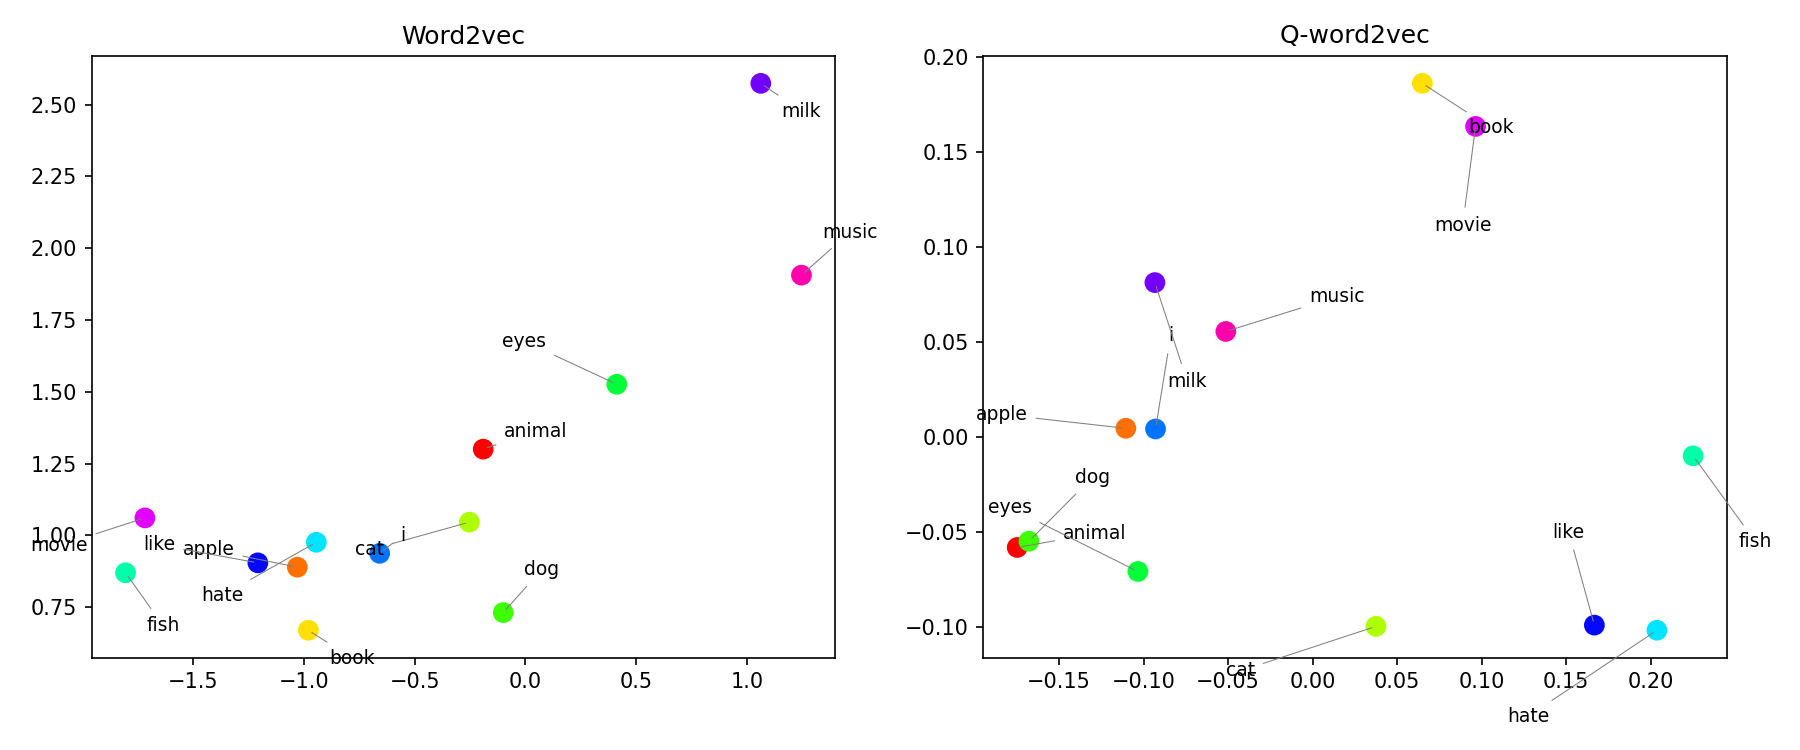
\includegraphics[width=0.95\linewidth]{imagenes/embeddings_comparison.png}
  \caption{Comparación de los \textit{embeddings} obtenidos por Word2Vec (izquierda) y QWord2Vec tras reducción dimensional mediante \gls{pca} (derecha). Cada punto representa una palabra del vocabulario, coloreada según su clúster semántico de referencia: animal, food, culture y sentiment.}
  \label{fig:embeddings_comparison}
\end{figure}

En los \textit{embeddings} de \textit{Word2Vec} se observan varias agrupaciones coherentes con los clústeres semánticos definidos como referencia. El par más fuerte de todo el vocabulario es \textit{book}--\textit{movie} con una similitud coseno de $0.998$, seguido por \textit{cat}--\textit{animal} ($0.962$), \textit{dog}--\textit{eyes} ($0.949$), \textit{i}--\textit{hate} ($0.930$) y \textit{apple}--\textit{milk} ($0.928$). Estos pares reflejan correctamente las co-ocurrencias dominantes del corpus y muestran que el modelo ha sido capaz de aprender, en términos generales, la estructura semántica esperada.

No obstante, también se aprecian relaciones que no se corresponden con la intuición semántica. Algunos pares del mismo clúster presentan similitudes inesperadamente bajas, como \textit{dog}--\textit{cat} ($0.326$) o \textit{music}--\textit{movie} ($0.276$), mientras que \textit{dog}--\textit{eyes} alcanza un valor muy alto ($0.949$) pese a que \textit{eyes} pertenece al clúster animal por una sola co-ocurrencia textual. La causa principal es el reducido tamaño del corpus, con tan pocas frases, las palabras frecuentes con muchos contextos distintos (como \textit{like}, \textit{i} o \textit{cat}) ven su vector dispersado en múltiples direcciones, dificultando que se acerquen a ningún término específico.

En los \textit{embeddings} de \textit{QWord2Vec}, los resultados proyectados muestran patrones también coherentes con las relaciones de co-ocurrencia del corpus, aunque organizados de forma distinta a los de Word2Vec. El par más cercano en la proyección \gls{pca} es \textit{dog}--\textit{animal}, con una distancia inferior a $0.013$, consistente con el hecho de que ambas palabras comparten los mismos dos contextos más frecuentes (\textit{cat} y \textit{like}). La palabra \textit{eyes} se sitúa próxima a este grupo (a unas $0.06$ unidades de \textit{dog} y \textit{animal}), mientras que \textit{cat} queda algo más alejada (en torno a $0.21$ unidades). El par \textit{like}--\textit{hate} también aparece muy próximo (alrededor de $0.044$) al compartir los mismos \textit{top}-$2$ contextos (\textit{i} y \textit{dog}), y \textit{book}--\textit{movie} muestra una distancia comparable ($\approx 0.053$), reflejando una agrupación parcial del clúster cultura.

\subsection{Similitud coseno}

Para complementar el análisis visual anterior y validarlo con mayor rigor, se presenta a continuación la matriz de similitud coseno entre todos los pares de palabras del vocabulario para cada modelo. A diferencia del gráfico de dispersión, esta métrica opera directamente sobre los vectores completos sin aplicar ninguna reducción dimensional, por lo que ofrece una visión más fiel de la estructura aprendida. Los valores se encuentran en el rango $[0, 1]$, donde $1$ indica máxima similitud y $0$ ausencia de relación.

\begin{figure}[h]
  \centering
  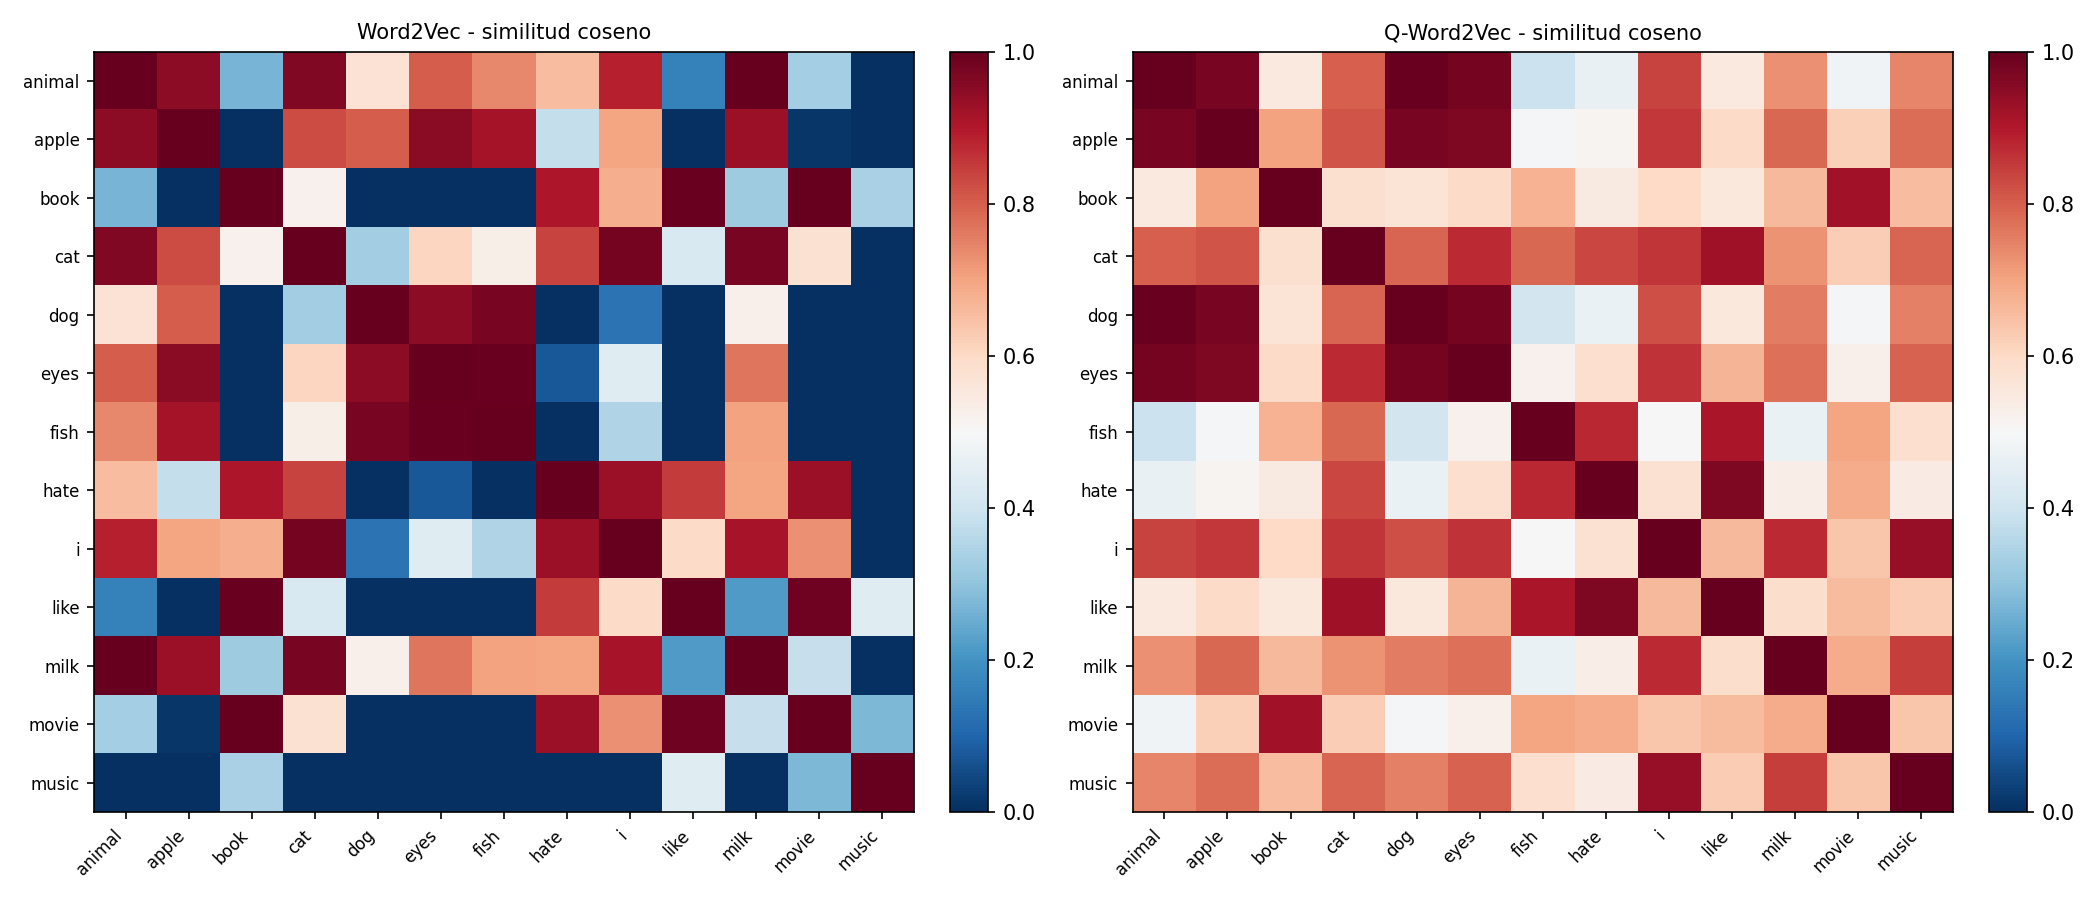
\includegraphics[width=0.95\linewidth]{imagenes/cosine_similarity_comparison.png}
  \caption{Matrices de similitud coseno para Word2Vec (izquierda) y Q-Word2Vec (derecha). Cada celda representa la similitud entre un par de palabras, donde el rojo indica alta similitud y el azul ausencia de relación.}
  \label{fig:cosine_similarity}
\end{figure}

Comenzando por los pares que ambos modelos coinciden en capturar con alta similitud, \textit{book}--\textit{movie} aparece como uno de los más fuertes en las dos representaciones, tal y como cabría esperar al pertenecer al mismo clúster semántico. \textit{Word2Vec} también obtiene similitudes elevadas en \textit{cat}--\textit{animal} ($0.962$), \textit{i}--\textit{hate} ($0.930$) y \textit{apple}--\textit{milk} ($0.928$), todas ellas relaciones intra-clúster.

Las diferencias más notables aparecen en el clúster de cultura. \textit{Word2Vec} captura con fuerza únicamente el par \textit{book}--\textit{movie} ($0.998$), mientras que las similitudes \textit{book}--\textit{music} ($0.338$) y \textit{music}--\textit{movie} ($0.276$) son sensiblemente bajas, dejando a \textit{music} prácticamente desconectada del resto del clúster. \textit{QWord2Vec}, en cambio, presenta una agrupación más equilibrada de las tres palabras de cultura, siendo el único modelo que refleja cierta cohesión simultánea entre \textit{book}, \textit{music} y \textit{movie}.

La situación se invierte parcialmente en el clúster de sentimiento. \textit{Word2Vec} agrupa con alta similitud los pares \textit{i}--\textit{hate} y \textit{like}--\textit{hate} ($0.930$ y $0.850$ respectivamente), aunque el par \textit{i}--\textit{like} resulta sorprendentemente más bajo ($0.596$) por la dispersión de contextos de la palabra \textit{like} en el corpus. \textit{QWord2Vec} reproduce con claridad el par \textit{like}--\textit{hate}, pero \textit{i} queda algo más desconectada de las otras dos. Esto es consecuencia directa sobre cómo se construyen las etiquetas en la versión cuántica. Al construir la etiqueta de \textit{i} a partir de sus dos contextos más frecuentes, se descartan otras co-ocurrencias menores que sí pueden ser útiles para reflejar la cercanía semántica con \textit{like} y \textit{hate}, esto sin embargo \textit{Word2Vec} sí que lo aprovecha.

\subsection{Correlación de Pearson y métricas finales}

Para cuantificar en qué medida ambos modelos organizan el espacio de palabras de forma parecida, se ha calculado el coeficiente de correlación de Pearson entre los vectores de distancias coseno de \textit{Word2Vec} y \textit{QWord2Vec}. El valor obtenido es de $0.2920$, lo que refleja una correlación baja entre las estructuras de similitud de ambos modelos, y sirve para evaluar de forma global cómo de parecida es la disposición de las palabras en ambos espacios. También es la principal magnitud comparativa del artículo de referencia \cite{ohno_qword2vec_2025}, en el que se obtiene un valor de $0.81$ sobre el mismo corpus, aunque cabe recordar que en dicho artículo se buscaba que ambas representaciones fueran lo más parecidas posibles.

Complementariamente, se reporta el \textit{cosine\_delta} final calculado sobre los \textit{embeddings} completos de cada modelo, sin aplicar reducción dimensional. \textit{Word2Vec} alcanza un \textit{cosine\_delta} de $0.8927$, que indica una clara separación entre los clústeres semánticos en el espacio euclídeo. \textit{QWord2Vec}, por su parte, obtiene un \textit{cosine\_delta} de $0.0550$ calculado directamente sobre los vectores de $2^4 = 16$ dimensiones del espacio de Hilbert. Este valor bajo refuerza la interpretación expresada durante el análisis visual: aunque la proyección \gls{pca} preservaba solo el $74.8\%$ de la varianza y las agrupaciones podían parecer razonables a primera vista, el \textit{cosine\_delta} calculado en el espacio completo confirma que los \textit{embeddings} cuánticos del primer corpus no capturan la estructura semántica de los clústeres de forma comparable a \textit{Word2Vec}.

\subsection{Discusión}

Los resultados obtenidos permiten extraer conclusiones relevantes en relación con el objetivo central de este trabajo.

En primer lugar, la baja correlación de Pearson ($0.2920$) no debe interpretarse como un fallo de ninguno de los dos modelos, sino como evidencia de que el espacio euclídeo y el espacio de Hilbert organizan la información semántica de forma diferente. \textit{Word2Vec} ha aprendido una geometría mediante la optimización directa sobre todos los pares de co-ocurrencia en el espacio euclídeo, y \textit{QWord2Vec} mediante la búsqueda de la distribución de probabilidad cuántica más cercana a los vectores de etiqueta en el espacio de Hilbert. Que ambas representaciones difieran en su estructura no contradice la validez semántica de ninguna de ellas.

En segundo lugar, el \textit{cosine\_delta} final permite comparar directamente la calidad semántica de ambas representaciones. \textit{Word2Vec} alcanza $0.8927$, indicando una separación clara entre los clústeres en el espacio euclídeo. \textit{QWord2Vec}, con un valor de $0.0550$, muestra que los \textit{embeddings} cuánticos obtenidos con este corpus no preservan la estructura semántica de los clústeres de forma comparable. Cabe destacar que el bajo \textit{cosine\_delta} no implica que el entrenamiento haya fracasado en todos los sentidos: el \textit{error rate} de $0.0769$ evidencia que el circuito ha aprendido a predecir correctamente los contextos más frecuentes de cada palabra. La discrepancia entre ambas métricas refleja que el espacio de Hilbert organiza la información de forma diferente al espacio euclídeo: el circuito consigue discriminar los pares (palabra, contexto) sin que ello se traduzca necesariamente en una agrupación por clústeres semánticos robusta medible mediante similitud coseno.

En cuanto a las limitaciones que condicionan estos resultados, cabe señalar tres factores principales. El primero es el tamaño y desequilibrio del corpus, con apenas 13 frases y un vocabulario de 13 palabras con una distribución de frecuencias muy desigual, las representaciones aprendidas por ambos modelos reflejan solo los patrones encontrados y no así una buena generalización del corpus. El segundo factor es la limitación inherente a la simulación clásica de circuitos cuánticos, que impone restricciones severas sobre el tamaño del experimento realizable (a mayor tamaño el tiempo de ejecución aumenta exponencialmente). Esto no permite acceder a las ventajas computacionales que la computación cuántica real podría ofrecer. El tercer factor es que el algoritmo utilizado \textit{Word2Vec} lleva 13 años de mejoras desde que se publicó mientras que la versión cuántica es de hace menos de 1 año (agosto de 2025), por lo que no se tiene aún las mejores herramientas posibles para sacarle un mayor provecho a este circuito al ser una primera versión básica.

En conjunto, los resultados de esta primera fase muestran que \textit{QWord2Vec} aprende a predecir los contextos más frecuentes de forma efectiva, pero los \textit{embeddings} resultantes no capturan la estructura semántica de los clústeres con la misma eficacia que \textit{Word2Vec}. Esta diferencia puede atribuirse tanto al tamaño y desequilibrio del corpus como a las propias características del espacio de Hilbert como representación semántica. La segunda fase de experimentación, con un corpus más equilibrado, permitirá evaluar si esta brecha se reduce al mejorar las condiciones de entrenamiento.


\section{Experimentación con corpus ampliado}
\label{sec:experimentacion-v2}

Una vez analizados los resultados obtenidos sobre el corpus inicial, se ha llevado a cabo una segunda fase de experimentación con el objetivo de evaluar principalmente en qué medida las limitaciones observadas son atribuibles al tamaño y al desequilibrio del corpus original. Esta segunda fase replica el procedimiento descrito sobre el primer corpus. El factor de diferencia es que ahora se utiliza un corpus ampliado, esto conlleva a realizar un reajuste de los hiperparámetros que requieren un nuevo equilibrio dada la modificación de las instancias de entrenamiento. Para evitar redundancias, esta sección describe únicamente los aspectos que cambian respecto a la primera versión del corpus utilizado, asumiendo el resto de la metodología, las métricas de evaluación y los criterios de parada ya definidos.

\subsection{Ampliación del corpus}

El nuevo corpus extiende el original hasta alcanzar las \textbf{64 frases}, manteniendo el mismo vocabulario de 13 palabras distintas. Las frases se han redistribuido de modo que cada uno de los cuatro clústeres definidos en la sección de entrenamiento (\textit{animal}, \textit{food}, \textit{culture} y \textit{sentiment}) reciba aproximadamente 16 frases, dando lugar a un corpus equilibrado en el que ningún clúster domina sobre los demás, evitando así el desbalanceo documentado del primer corpus utilizado.

Este equilibrio resulta beneficioso para ambos modelos. En \textit{Word2Vec} evita que los pares de co-ocurrencia procedentes del clúster más numeroso dominen sobre el resto. En \textit{QWord2Vec}, donde los vectores de etiqueta se construyen a partir de los dos contextos más frecuentes de cada palabra, una distribución de frases más uniforme genera etiquetas más representativas del vocabulario completo y reduce los sesgos hacia palabras con mayor frecuencia que el resto.

\subsection{Reajuste de hiperparámetros}

Debido al cambio en la cantidad y diversidad de las instancias de entrenamiento, se reevaluó los hiperparámetros de ambos modelos. En consecuencia, se ha repetido el procedimiento de \textit{Grid Search} descrito previamente, manteniendo los mismos rangos generales y aplicando ajustes locales en torno a los valores que resultaron óptimos en la fase inicial.

En el caso de \textbf{Word2Vec}, la nueva configuración óptima es:

\begin{itemize}
  \item \textit{vector\_size} $= 4$ (frente a $2$ en la fase inicial).
  \item \textit{window} $= 2$ (sin cambios).
  \item \textit{alpha} $= 0.068$ (frente a $0.59$).
  \item \textit{negative} $= 2$ (sin cambios).
  \item \textit{ns\_exponent} $= 0.4$ (frente a $0.0$).
  \item \textit{epochs} $= 400$ (frente a $500$).
\end{itemize}

El cambio más significativo es la reducción drástica de la tasa de aprendizaje inicial. En la fase anterior, el reducido tamaño del corpus exigía pasos de gradiente agresivos para escapar de mínimos locales y aprovechar al máximo cada época. Con 64 frases y al tener poca diversidad de palabras (solo 13), el modelo recibe una señal mucho más rica por época y converge con un \textit{alpha} considerablemente más suave, lo que se traduce en una optimización más estable y menos errática. El aumento de \textit{vector\_size} de $2$ a $4$ es debido a que con mayor número de instancias de entrenamiento se requiere aprender un mayor número de características para diferenciar correctamente. Es decir, con 13 frases una dimensionalidad mayor habría provocado sobreajuste, mientras que con 64 frases existe señal suficiente para separar las palabras en el espacio de cuatro dimensiones de forma significativa y precisa. Para preservar la posibilidad de visualizar los \textit{embeddings} en el plano se aplica posteriormente \gls{pca} sobre las cuatro dimensiones, conservando una varianza en torno al $86,2\%$. Por último, el cambio en \textit{ns\_exponent} de $0.0$ a $0.4$ refleja que, al equilibrarse el corpus, ya no resulta necesario forzar una distribución uniforme de muestras negativas para compensar el desequilibrio léxico, siendo más adecuado un valor intermedio que conserve cierta proporcionalidad con la frecuencia real de cada palabra.

En el caso de \textbf{QWord2Vec}, el \textit{Grid Search} se aplicó sobre el mismo espacio de hiperparámetros que en la fase inicial, pero el único valor que resultó modificado fue el parámetro $C$ de la función de pérdida, que pondera la contribución del coeficiente de correlación de Pearson frente a la entropía cruzada. La búsqueda exploró los valores $C \in \{1, 2, 3, 4\}$, seleccionándose finalmente $C = 3$ frente al $C = 2$ utilizado en la fase inicial. Un valor mayor de $C$ penaliza con más fuerza la falta de correlación entre la distribución de las palabras en el espacio de Hilbert y las etiquetas de entrenamiento establecidas. Con un corpus más amplio y rico en co-ocurrencias, la señal de correlación es más fiable y soporta mejor penalización adicional sin desestabilizar el entrenamiento pero a la vez consiguiendo una mejor representación de los embeddings en el espacio de Hilbert. El resto de hiperparámetros del optimizador \gls{qn-spsa} se mantiene sin cambios respecto a la fase inicial, ya que la búsqueda no encontró configuraciones mejores al variarlos.

\subsection{Resultados de Word2Vec}

La Figura \ref{fig:loss_curves_word2vec_v2} muestra la evolución del entrenamiento de \textit{Word2Vec} sobre el corpus ampliado. La curva de \textit{cosine\_delta} presenta una tendencia ascendente claramente más estable que en la fase inicial, alcanzando el mejor punto en la época 341 exactamente con un valor de $0.9360$. La pérdida de \textit{Negative Sampling} mantiene cierto grado de oscilación, comportamiento esperable dada su naturaleza estocástica así como el problema de condición de carrera del que carece explicado con anterioridad.

\begin{figure}[h]
  \centering
  
\includegraphics[width=1.0\linewidth]{imagenes/lossCurvesWord2Vec_v2.png}
  \caption{Evolución del \textit{cosine\_delta} (eje izquierdo) y de la pérdida de \textit{Negative Sampling} (eje derecho) durante el entrenamiento de \textit{Word2Vec} sobre el corpus ampliado.}
  \label{fig:loss_curves_word2vec_v2}
\end{figure}

El valor final de \textit{cosine\_delta} mejora en $+0.0433$ puntos respecto a la fase inicial ($0.9360$ frente a $0.8927$), confirmando que el aumento del corpus se traduce en una mejor agrupación semántica del vocabulario. La Figura \ref{fig:embeddings_word2vec_v2} representa los \textit{embeddings} resultantes reducido a dos dimensiones mediante la técnica de \gls{pca}.

\begin{figure}[h]
  \centering
  
\includegraphics[width=1.0\linewidth]{imagenes/embeddingsWord2Vec_v2.png}
  \caption{Visualización de los \textit{embeddings} de \textit{Word2Vec} obtenidos con el corpus ampliado, proyectados sobre las dos primeras dimensiones del espacio de \textit{embedding}. Cada palabra se colorea según su clúster semántico de referencia.}
  \label{fig:embeddings_word2vec_v2}
\end{figure}

Como se aprecia en la Figura \ref{fig:embeddings_comparison_v2} a pesar de haber aplicado el \gls{pca} perdiendo información importante, están bien representados los cuatro clusters definidos mediante la similitud coseno (\textit{animal}, \textit{food}, \textit{culture} y \textit{sentiment}). Con esto se aprecia que a pesar de haber habido una pequeño incremento en el \textit{cosine\_delta} final, visualmente ha habido una mejora clara en cuanto a la separación de los embeddings entre los clusters.

El análisis de las similitudes coseno por pares dentro de cada clúster, mostrado en la Figura \ref{fig:cosine_similarity_v2}, revela una mejora notable en la cohesión interna de la mayoría de los grupos. La diferencia más relevante respecto al corpus inicial es que se ha acentuado el contraste entre las dos regiones de la matriz, las celdas asociadas a pares disimilares se han desplazado hacia valores aún más bajos, mientras que las celdas correspondientes a pares del mismo clúster han ganado en intensidad. Es decir, al disponer de un mayor número de instancias de entrenamiento, el modelo ha sido capaz simultáneamente de discriminar mejor entre clústeres distintos y de reforzar la cohesión interna de cada uno de ellos. Esta tendencia se refleja con claridad en los valores numéricos por clúster. En el clúster \textit{animal}, los pares \textit{dog}--\textit{cat} y \textit{dog}--\textit{animal} aumentan su similitud desde $0.326$ y $0.572$ hasta $0.789$ y $0.916$ respectivamente. En el clúster \textit{food}, el par \textit{fish}--\textit{milk} pasa de $0.702$ a $0.953$, mientras que \textit{apple}--\textit{fish} se mantiene en torno a $0.914$. Por último, en el clúster \textit{culture}, el par \textit{music}--\textit{movie} mejora de forma drástica de $0.276$ a $0.934$, recuperando la cohesión que en la fase inicial se concentraba artificialmente en \textit{book}--\textit{movie}.

\begin{figure}[h]
  \centering
  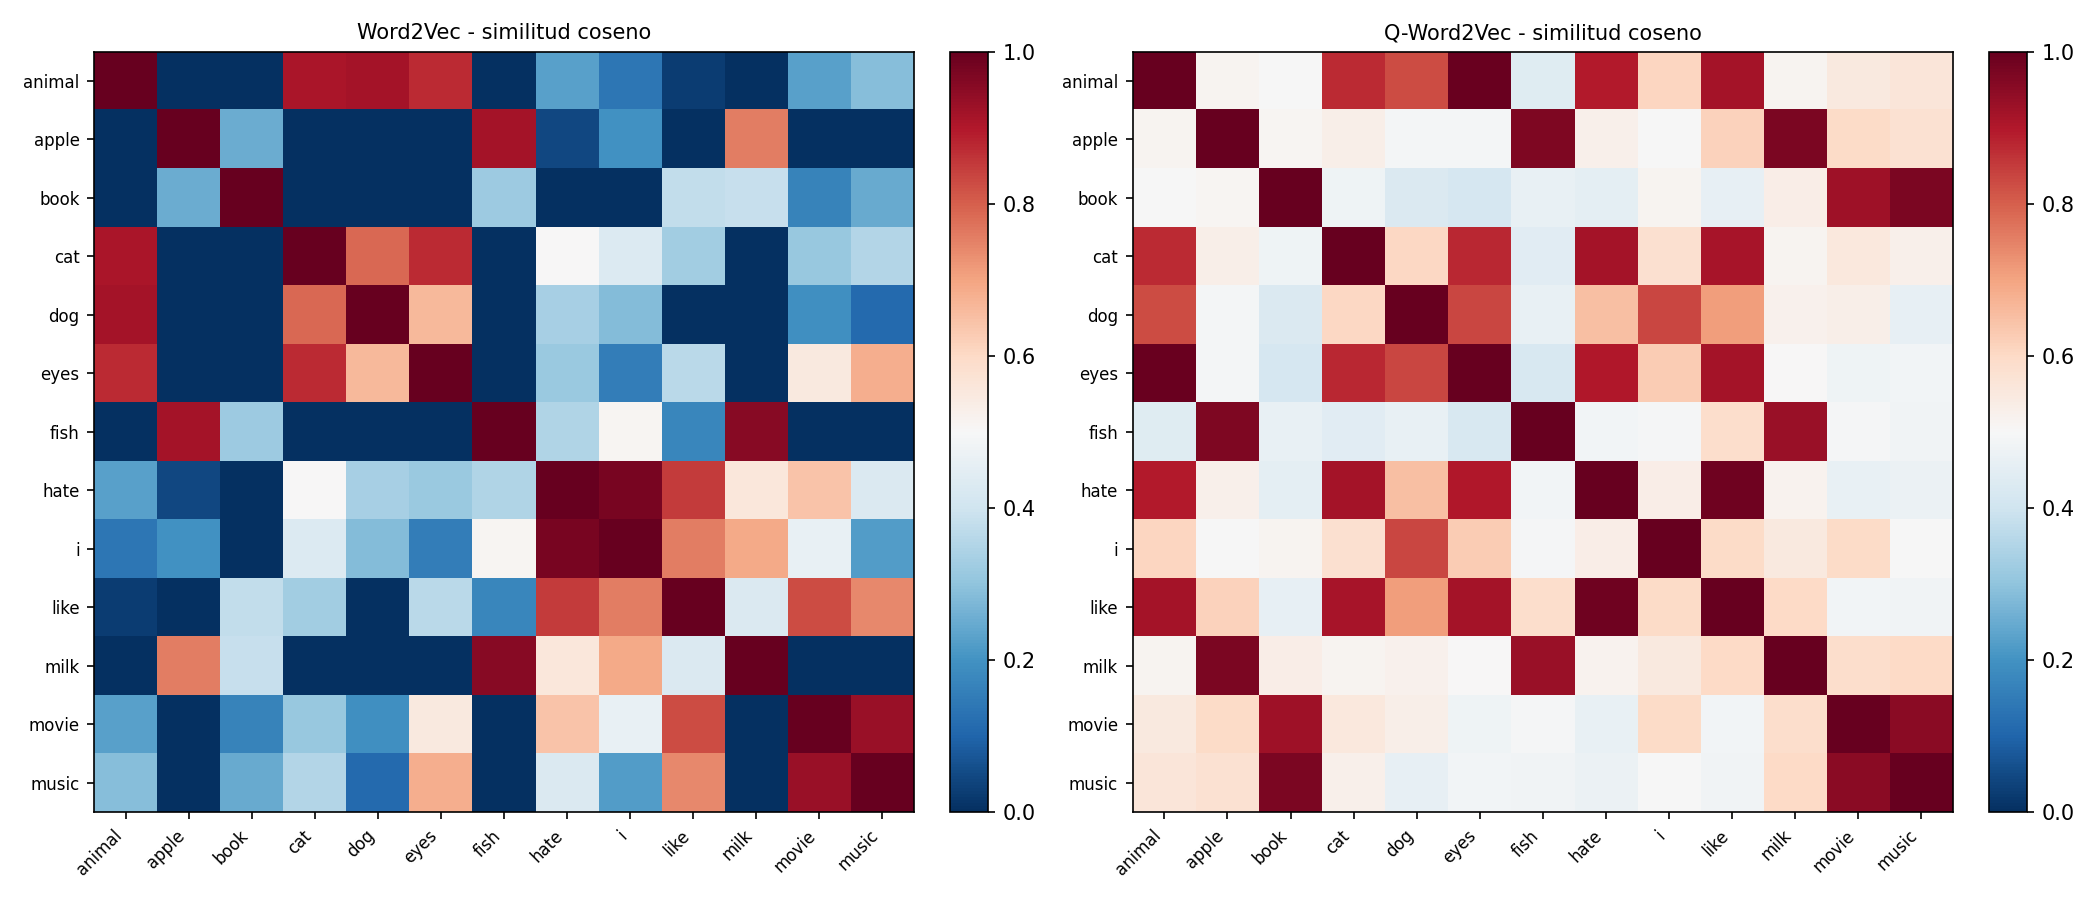
\includegraphics[width=1.0\linewidth]{imagenes/cosine_similarity_comparison_v2.png}
  \caption{Matrices de similitud coseno para \textit{Word2Vec} (izquierda) y \textit{QWord2Vec} (derecha) entrenados con el corpus ampliado.}
  \label{fig:cosine_similarity_v2}
\end{figure}

La excepción más llamativa es el par \textit{book}--\textit{movie}, que retrocede de $0.998$ a $0.167$, junto con el par \textit{book}--\textit{music}, que se mantiene en un valor también bajo de $0.248$. Esta caída no responde a una diferencia significativa en las co-ocurrencias entre las tres palabras del clúster \textit{culture} (\textit{book}, \textit{music} y \textit{movie}) aparecen en el corpus ampliado un número de veces juntas muy similar entre sí, por lo que el conteo de frecuencias por sí solo no permite justificar la disparidad observada. La causa más probable se encuentra en la selección estocástica de muestras negativas que realiza \textit{Negative Sampling}, junto con el carácter no determinista del propio optimizador, puede empujar a palabras del mismo clúster en direcciones distintas cuando se seleccionan unas como negativas de otras. La configuración finalmente aprendida concentra la cohesión interna del clúster cultura en el par \textit{music}--\textit{movie} (similitud $0.934$) y desplaza a \textit{book} hacia una dirección distinta, hipotéticamente influida por sus co-ocurrencias adicionales con palabras del clúster \textit{sentiment} a través de frases como \textit{i like book} o \textit{i hate book}. Esta solución resulta globalmente óptima en términos de \textit{cosine\_delta}, aun a costa de penalizar un par concreto del mismo clúster.

\subsection{Resultados de QWord2Vec}

El entrenamiento de \textit{QWord2Vec} sobre el corpus ampliado y con la nueva configuración alcanza un \textit{error rate} de $0.1154$ en la mejor iteración. El mejor punto se localiza en torno a la iteración 400 sobre un total de 800 (debido a la tardía parada del \textit{Early Stopping}), a partir de la cual la optimización oscila sin mejora adicional, comportamiento habitual de \gls{qn-spsa} en espacios de alta dimensión con pocos datos. A partir de los \textit{embeddings} correspondientes a dicha mejor época se calcula el \textit{cosine\_delta} sobre los vectores completos de $16$ dimensiones, que alcanza un valor de $0.3293$, frente al $0.0550$ obtenido con el primer corpus. La correlación de Pearson final entre las distancias coseno de \textit{Word2Vec} y \textit{QWord2Vec} se sitúa en $0.4940$, valor inferior al $0.81$ reportado por el trabajo de referencia \cite{ohno_qword2vec_2025} pero superior al obtenido con el primer corpus inicial y desbalanceado utilizado. La Figura \ref{fig:loss_curves_qword2vec_v2} muestra la evolución conjunta de la función de pérdida y del \textit{error rate} durante el entrenamiento.

\begin{figure}[h]
  \centering
  
\includegraphics[width=0.85\linewidth]{imagenes/lossCurvesQWord2Vec_v2.png}
  \caption{Evolución de la función de pérdida (eje izquierdo) y del \textit{error rate} (eje derecho) durante el entrenamiento de \textit{QWord2Vec} sobre el corpus ampliado.}
  \label{fig:loss_curves_qword2vec_v2}
\end{figure}

La Figura \ref{fig:embeddings_comparison_v2} muestra la proyección \gls{pca} de las distribuciones de probabilidad de los \textit{embeddings} cuánticos junto a los de \textit{Word2Vec}, con una varianza explicada del $72.5\%$, similar a la obtenida en la fase inicial. La separación entre clústeres es claramente mejor que en la versión inicial. Los clusters de \textit{culture} y de \textit{food} están correctamente separados y bien representados por las palabras que los componen. Sin embargo los clusters de \textit{animal} y \textit{sentiment} se encuentran uno superpuesto con otro. Esto principalmente puede deberse a la reducción de dimensionalidad con la pérdida de varianza tan grande que se tiene. A pesar de ello, es una clara mejora visual respecto a la primera versión de corpus.

\begin{figure}[h]
  \centering
  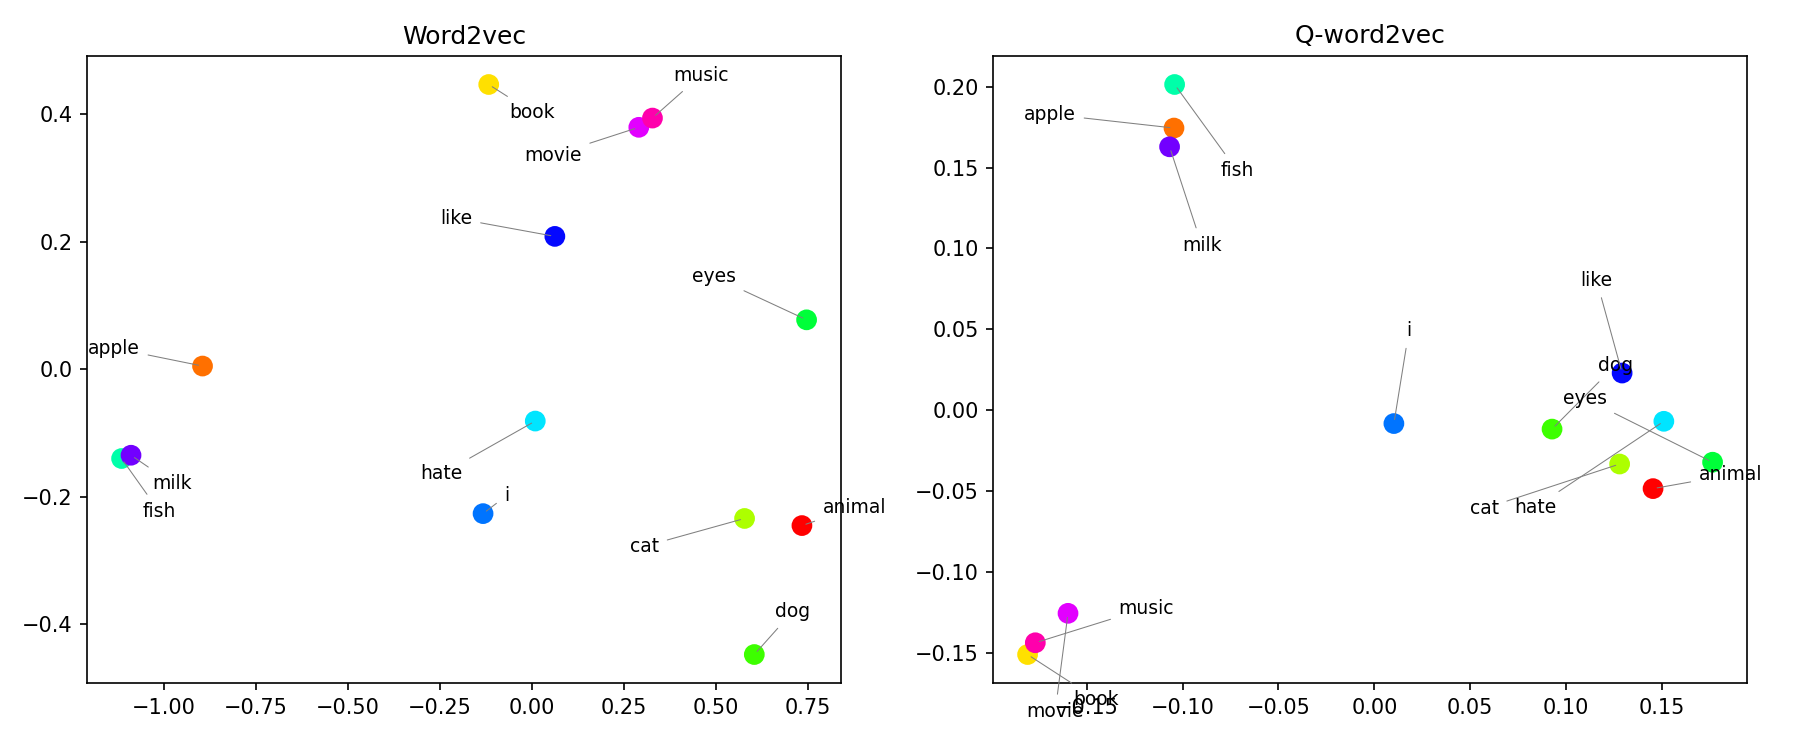
\includegraphics[width=1.0\linewidth]{imagenes/embeddings_comparison_v2.png}
  \caption{Comparación de los \textit{embeddings} de \textit{Word2Vec} (izquierda) y \textit{QWord2Vec} (derecha) entrenados con el corpus ampliado. Para \textit{QWord2Vec} se aplica \gls{pca} sobre las distribuciones de probabilidad de dimensión $2^4 = 16$.}
  \label{fig:embeddings_comparison_v2}
\end{figure}

\subsection{Comparación entre fases}

La Tabla \ref{tab:comparacion_v1_v2} sintetiza las principales métricas de \textit{Word2Vec} en ambas fases.

\begin{table}[h]
  \centering
  \begin{tabular}{|l|c|c|c|}
    \hline
    \textbf{Métrica}               & \textbf{Fase inicial} & \textbf{Corpus ampliado} & $\Delta$ \\
    \hline
    \textit{cosine\_delta} final   & $0.8927$              & $0.9360$                 & $+0.043$ \\
    \textit{dog}--\textit{cat}     & $0.326$               & $0.789$                  & $+0.463$ \\
    \textit{dog}--\textit{animal}  & $0.572$               & $0.916$                  & $+0.344$ \\
    \textit{cat}--\textit{animal}  & $0.962$               & $0.910$                  & $-0.052$ \\
    \textit{fish}--\textit{milk}   & $0.702$               & $0.953$                  & $+0.251$ \\
    \textit{music}--\textit{movie} & $0.276$               & $0.934$                  & $+0.658$ \\
    \textit{book}--\textit{movie}  & $0.998$               & $0.167$                  & $-0.831$ \\
    \hline
  \end{tabular}
  \caption{Comparación de las similitudes coseno intra-clúster más relevantes y del \textit{cosine\_delta} global entre las dos fases de experimentación de \textit{Word2Vec}.}
  \label{tab:comparacion_v1_v2}
\end{table}

La mejora es generalizada en la mayoría de los pares intra-clúster. Las únicas métricas que retroceden corresponden a casos en los que la fase inicial había generado relaciones elevadas debido al desequilibrio del corpus.

En el caso de \textit{QWord2Vec} pueden destacarse tres observaciones. En primer lugar, el \textit{error rate} de entrenamiento aumenta de $0.0769$ a $0.1154$, lo que refleja que el corpus ampliado introduce un mayor número de co-ocurrencias distintas que el circuito debe discriminar, haciendo la tarea intrínsecamente más exigente con la misma capacidad expresiva del circuito. Sin embargo, el \textit{cosine\_delta} mejora de forma muy significativa de $0.0550$ a $0.3293$, lo que indica que los \textit{embeddings} cuánticos de la segunda fase capturan la estructura semántica de los clústeres de forma notablemente mejor que en la primera. En segundo lugar, la separación visual entre clústeres en la proyección \gls{pca} es notablemente más nítida en la segunda fase, especialmente para los grupos \textit{food} y \textit{culture}, que en la fase inicial aparecían más solapados. En tercer lugar, la correlación de Pearson aumenta de $0.2920$ a $0.4940$, lo que indica una mejor alineación entre la geometría aprendida por el circuito cuántico y la del modelo clásico, aunque sigue siendo inferior al $0.81$ reportado en el trabajo de referencia \cite{ohno_qword2vec_2025}.

La interpretación conjunta de estos resultados es que, al ampliar el corpus, el modelo cuántico reduce la precisión en la predicción de los contextos más frecuentes por palabra (el \textit{error rate} aumenta), a cambio de una representación globalmente más coherente con la estructura semántica del corpus (el \textit{cosine\_delta} mejora de $0.0550$ a $0.3293$). Aunque el \textit{cosine\_delta} de $0.3293$ sigue siendo notablemente inferior al de \textit{Word2Vec} con corpus ampliado ($0.9360$), la mejora relativa es sustancial y sugiere que la calidad de los \textit{embeddings} cuánticos es especialmente sensible al equilibrio del corpus de entrenamiento. En conjunto, la segunda fase confirma que ambos modelos se benefician de un corpus equilibrado, siendo \textit{Word2Vec} el que mantiene una mayor calidad numérica y \textit{QWord2Vec} el que experimenta la mejora relativa más pronunciada en la organización del espacio de Hilbert.


\section{Análisis de tiempos de ejecución}

Además de la calidad semántica de los \textit{embeddings}, el coste computacional constituye un factor determinante a la hora de evaluar la viabilidad práctica de ambos modelos. Los tiempos que se comentarán a continuación se han medido desde el inicio del entrenamiento, excluyendo cualquier preprocesamiento previo, y se han obtenido ejecutando cada algoritmo en las condiciones descritas en la sección de entorno de ejecución, minimizando la interferencia de otros procesos del sistema para que así dispongan del mayor rendimiento posible. Se realizaron varias ejecuciones para verificar la consistencia de los resultados. Los valores obtenidos son prácticamente idénticos en las dos fases de experimentación descritas, dado que el aumento del corpus de 13 a 64 frases no modifica los factores que dominan el coste de cada modelo. Por ello, los tiempos se reportan de forma conjunta para ambas fases.

\textit{Word2Vec} completa el entrenamiento en aproximadamente \textbf{1 segundo} en las dos fases. Este tiempo reducido se explica por dos factores principales. Por un lado, el corpus utilizado es notablemente pequeño en comparación con los conjuntos de datos para los que este tipo de modelos fue diseñado, que habitualmente comprenden cientos de miles de palabras únicas y millones de frases. Por otro lado, \textit{Negative Sampling} actualiza únicamente un subconjunto reducido de pesos por iteración, en lugar de recalcular la salida sobre todo el vocabulario. La principal fuente de sobrecarga adicional es la evaluación periódica del \textit{cosine\_delta}, necesaria para el mecanismo de \textit{Best Model Checkpointing}, aunque su impacto sobre el tiempo total es marginal dada la brevedad del entrenamiento y lo sencillo que es computacionalmente calcular esta métrica adicional. El paso de 13 a 64 frases multiplica el número de pares (palabra, contexto) procesados por época, pero el coste por par es tan bajo que la diferencia resulta imperceptible a escala de segundo.

\textit{QWord2Vec}, por su parte, requiere aproximadamente \textbf{50 minutos} para completar el entrenamiento, también en ambas fases. Esta diferencia de tiempo tan grande respecto a \textit{Word2Vec} se debe a la acumulación de varios factores inherentes a la simulación clásica de circuitos cuánticos. El principal cuello de botella es la evaluación de la función de pérdida. En cada llamada se transpilan y simulan los 13 circuitos cuánticos del vocabulario con 2048 \textit{shots} por circuito mediante \textit{AerSimulator}. La simulación clásica de circuitos cuánticos es costosa por naturaleza, ya que el espacio de estados crece exponencialmente con el número de qubits. Es importante señalar que el coste por iteración depende del tamaño del vocabulario y no del número de frases del corpus, por lo que la ampliación de la fase inicial a la segunda fase no incrementa el tiempo de entrenamiento.

A este coste base se añaden las múltiples evaluaciones de la función de pérdida que \gls{qn-spsa} requiere por iteración para estimar simultáneamente el gradiente y el hessiano. Con un valor de \textit{resamplings} de 5 y un \textit{hessian delay} de 400, cada iteración genera 10 llamadas adicionales al circuito (2 necesarias para el tensor métrico de Fubini-Study por 5 \textit{resamplings} para calcular la media obtenida) para estimar la información geométrica del espacio de parámetros. Adicionalmente, la estrategia de inicialización por \textit{educated guess} introduce 10 evaluaciones previas al inicio del entrenamiento para seleccionar el mejor punto de partida. Por último, el mecanismo de \textit{Early Stopping}, configurado para evaluar el \textit{error rate} cada 10 iteraciones, añade un \textit{forward pass} completo sobre todo el vocabulario en cada comprobación, lo cual contribuye también al tiempo total de ejecución.

En conjunto, la diferencia de tiempos entre ambos modelos no se debe a una mayor complejidad algorítmica intrínseca de \textit{QWord2Vec}, sino a las limitaciones actuales de los simuladores clásicos para circuitos cuánticos. \textit{Word2Vec} opera directamente sobre matrices pequeñas ejecutadas en CPU (no requiere de tanto tiempo de computación) mediante gradiente estocástico, sin ninguna capa de simulación intermedia, lo que lo hace varias órdenes de magnitud más eficiente en el hardware disponible. Quizás si se ejecutara esto mismo en un entorno de computación cuántica real (como por ejemplo un dispositivo \gls{nisq}), podría reducirse el tiempo de entrenamiento considerablemente.

Los resultados obtenidos con ambos corpus utilizados, permiten realizar un diagnóstico del estado actual de los dos modelos. \textit{Word2Vec} demuestra una calidad semántica sólida y un coste computacional mínimo en las condiciones experimentales descritas, consolidándose como el modelo de referencia esperado. \textit{QWord2Vec}, por su parte, aprende representaciones coherentes en el espacio de Hilbert y mejora de forma significativa al equilibrar el corpus, aunque su \textit{cosine\_delta} y sus tiempos de ejecución quedan notablemente por debajo de los del modelo clásico bajo simulación. El capítulo siguiente interpreta estos resultados en el contexto de los objetivos planteados al inicio del trabajo, valora las implicaciones de las limitaciones identificadas y propone las líneas de investigación para seguir mejorando lo realizado aquí.
